\documentclass[a4paper]{article}
\usepackage[pdftex]{hyperref}
\usepackage[latin1]{inputenc}
\usepackage[english]{babel}
\usepackage{a4wide}
\usepackage{amsmath}
\usepackage{amssymb}
\usepackage{algorithmic}
\usepackage{algorithm}
\usepackage{ifthen}
\usepackage{listings}
% move the asterisk at the right position
\lstset{basicstyle=\ttfamily,tabsize=4,literate={*}{${}^*{}$}1}
%\lstset{language=C,basicstyle=\ttfamily}
\usepackage{moreverb}
\usepackage{palatino}
\usepackage{multicol}
\usepackage{tabularx}
\usepackage{comment}
\usepackage{verbatim}
\usepackage{color}


%% pdflatex?
\newif\ifpdf
\ifx\pdfoutput\undefined
\pdffalse % we are not running PDFLaTeX
\else
\pdfoutput=1 % we are running PDFLaTeX
\pdftrue
\fi
\ifpdf
\usepackage[pdftex]{graphicx}
\else
\usepackage{graphicx}
\fi
\ifpdf
\DeclareGraphicsExtensions{.pdf, .jpg}
\else
\DeclareGraphicsExtensions{.eps, .jpg}
\fi

\parindent=0cm
\parskip=0cm

\setlength{\columnseprule}{0.4pt}
\addtolength{\columnsep}{2pt}

\addtolength{\textheight}{5.5cm}
\addtolength{\topmargin}{-26mm}
\pagestyle{empty}

%%
%% Sheet setup
%% 
\newcommand{\coursename}{Machine Learning}
\newcommand{\courseno}{CO22-320372}
 
\newcommand{\sheettitle}{Mini-Project}
\newcommand{\mytitle}{}
\newcommand{\mytoday}{{April 20}, 2019}

% Current Assignment number
\newcounter{assignmentno}
\setcounter{assignmentno}{2}

% Current Problem number, should always start at 1
\newcounter{problemno}
\setcounter{problemno}{1}

%%
%% problem and bonus environment
%%
\newcounter{probcalc}
\newcommand{\problem}[2]{
  \pagebreak[2]
  \setcounter{probcalc}{#2}
  ~\\
  {\large \textbf{Problem {\arabic{assignmentno}}.{\arabic{problemno}}} \hspace{0.2cm}\textit{#1}} \refstepcounter{problemno}\vspace{2pt}\\}

\newcommand{\bonus}[2]{
  \pagebreak[2]
  \setcounter{probcalc}{#2}
  ~\\
  {\large \textbf{Bonus Problem {\arabic{assignmentno}}.{\arabic{problemno}}} \hspace{0.2cm}\textit{#1}} \refstepcounter{problemno}\vspace{2pt}\\}

%% some counters  
\newcommand{\assignment}{\arabic{assignmentno}}

%% solution  
\newcommand{\solution}{\pagebreak[2]{\bf Solution:}\\}

%% Hyperref Setup
\hypersetup{pdftitle={Homework \assignment},
  pdfsubject={\coursename},
  pdfauthor={},
  pdfcreator={},
  pdfkeywords={Computer Networks},
  %  pdfpagemode={FullScreen},
  %colorlinks=true,
  %bookmarks=true,
  %hyperindex=true,
  bookmarksopen=false,
  bookmarksnumbered=true,
  breaklinks=true,
  %urlcolor=darkblue
  urlbordercolor={0 0 0.7}
}

\begin{document}
\coursename \hfill Course: \courseno\\
Jacobs University Bremen \hfill \mytoday\\
{Dragi Kamov \\
Aadil Anil Kumar}\hfill
\vspace*{0.3cm}\\
\begin{center}
{\Large \sheettitle{} {\assignment}\\}
\end{center}

\textbf{{\Large Introduction}} \\ 

In the following document we aim to train a classifier for the digits dataset using a linear regression model combined with pricipal component analysis to reduce the dimensionality of the input patterns. After training the classifier we will set up a cross-validation scheme with which we will compare the different Mean Square Errors and Misclassification rates for the training and validation sets.  \\ \\ 

\textbf{{\Large 1 Dimensionality}} \\ 

\textbf{{\large 1.1 Feature Extraction}} \\

Feature extraction is a dimensionality reduction process used in machine learning to derive values (features) that are important from a dataset and thus reduce it to more manageable groups for processing. \\

\textbf{{\large 1.2 Types of Features}} \\

There are three main types of features: 
\begin{itemize}
\item K-means based features are features that group a collection of data points into related clusters  $C_1,...,C_K$ , each of them being represented by a codebook vector  $c_i$.
\item Hand-made features are referring to properties derived from human insight on information that is in the images.
\item Principal Component Analysis (PCA) is a feature that reduces the dimensionality of a data set consisting of many variables correlated with each other, while retaining the variation present in the dataset, up to the maximum extent. \\
\end{itemize}

\textbf{{\large 1.3 Principal Component Analysis}} \\

PCA in and of itself is a unsupervised learning algorithm, it aims to reduce the dimensionality of a given dataset to a k set of features while retaining the variation present in the dataset. The algorithm does so searching for a relationship between the datapoints and then quantifying the relationship by finding a list of principal axes in the data. \\ \\
The input patterns for the digits data set have a dimensionality of $\mathbb{R}^{240}$. This is simply too high to effectively make a model. Hence, we make use of the PCA algorithm to reduce the dimensionality of the input patterns to to $\mathbb{R}^{k}$. \\
\\

\textbf{{\Large 2 Linear Regression Implementation}} \\ 

\textbf{{\large 2.1 Preliminary Steps}} \\ 

\textbf{2.1.1 Adding Bias} \\

We first create a function to add a bias term to all the features. Linear Regression creates a model based on a offine function, which contains a bias term. Without the bias term we can only approximate the data using a linear function, leading to a ineffective model. \\


\textbf{2.1.1 One-hot Encoding} \\

Due the digits dataset not containing any kind of label, we generate class vectors for each label $\{0,1,...,10\}$ as $v \in \mathbb{R}^{10}$. \\

\begin{lstlisting}
function one-hot-encode (digit):
    rst = [0] * 10
    rst[digit] = 1
    return rst 
\end{lstlisting}
\qquad \\

\textbf{{\large 2.2 Linear Regression}} \\

For a given the given dataset and a fixed number of k features, our linear regression algorithm proceeds as follows: 
\begin{enumerate}
\item  Performing a PCA algorithm to reduce the dimensions of $data$ from $\mathbb{R}^{240}$ to $\mathbb{R}^{k}$. Thus, we can view PCA algorithms as a function $PCA: \mathbb{R}^{240} \to \mathbb{R}^{k}$
\item Split the entire dataset after dimension reduction into training set features $X \in \mathbb{R}^{1000 \times k}$ and test set features $X_{test} \in \mathbb{R}^{1000 \times k}$
\item Associate $X$ and $X_{test}$ with bias term, thus we have $X, X_{test} \in \mathbb{R}^{1000 \times (K + 1)}$
\item Build the correct class vector for training set as $Y \in \mathbb{R}^{(k + 1) \times 10}$ and test set as $Y_{test} \in \mathbb{R}^{(k + 1) \times 10}$. After such operation, we obtained the complete training set as $(X, Y)$ and the test set as $(X_{test}, Y_{test})$
\item Using the training set, compute the optimal weight matrix as 
$$ {W_{opt}}^\top = (\frac{1}{N} \cdot X \cdot X^\top + \alpha^2 \cdot I_{nxn})^{-1} \cdot \frac{1}{N} \cdot X \cdot Y $$
we can rewrite this as 
$$ W_{opt} = ((\frac{1}{N} \cdot X \cdot X^\top + \alpha^2 \cdot I_{nxn})^{-1} \cdot \frac{1}{N} \cdot X \cdot Y)^\top $$
\item Calculate the error term. \\
First, make a prediction: 
$$ Y_{pred} = (W_{opt} \cdot X)^\top $$
$$ Y_{test}pred = (W_{opt} \cdot X_{test})^\top $$
Using the prediction, we calculate the corresponding error:
$$ MSE_{train} = \frac{\|Y - Ypred\|^2}{1000} $$
$$ MSE_{test} = \frac{\|Ytest - Y_{test}pred\|^2}{1000} $$
$$ MISS_{train} = \frac{\sum_{i = 1}^{1000} \min(1, \|\arg\max(Y_i) - \arg\max(Ypred_i)\|)}{1000} $$
$$ MISS_{test} = \frac{\sum_{i = 1}^{1000} \min(1, \|\arg\max({Y_{test}}_i) - \arg\max(Y_{test}pred_i)\|)}{1000} $$ \\ 
\end{enumerate}

We use plain linear regression with $\alpha$ set to zero. \\ \\
\newpage
\textbf{{\Large 3 Analysis}} \\ 

First, we variate the value of k (features) and check to see how this in turn affects our error terms. \\

\textbf{Linear Plot} \\ \\
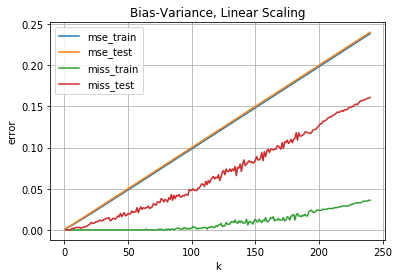
\includegraphics[scale=.95]{./1.png} \\ 
As you can see from figure 1, the MSE's for train and test do not vary much. While misclassification rate of train is a lot lower than that of test. \\

Now we use a log-log scaling of the data for the plot. \\ \\
\textbf{Log-Log Plot} \\ \\
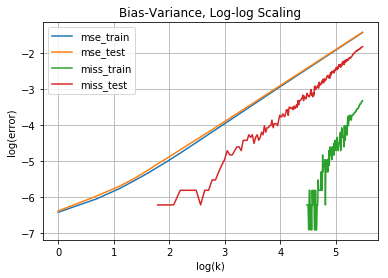
\includegraphics[scale=.95]{2.png}


\end{document}